\documentclass[landscape]{slides}
\usepackage[landscape]{geometry}
\usepackage{color}
\usepackage{amsfonts}
\usepackage{graphicx}
\usepackage[MeX]{polski}

\begin{document}
\begin{slide}
\centering
\textcolor{blue}{\Large{Karabin}}
\begin{itemize}
\item{Steyr AUG-77 (AUG – niem. Armee Universal Gewehr) (inna nazwa StG 77 – niem. Sturmgewehr 77) – austriacki uniwersalny karabin wojskowy zaprojektowany i produkowany od 1978 roku w firmie Steyr-Daimler-Puch – zaklad Steyr-Mannlicher GmbH und Com. KG. w Kleinraming. Zbudowany w ukladzie bullpup.}
\end{itemize}
\footnote{Zrodlo: Wikipedia}
\end{slide}


\begin{slide}
\begin{flushleft}
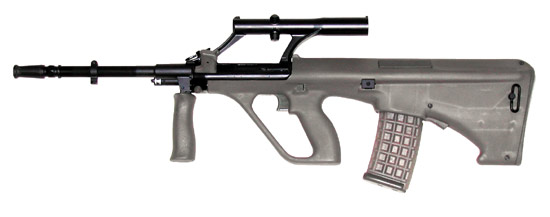
\includegraphics[width=3.5cm, angle=-10]{kaabin.jpg}
\end{flushleft}
\end{slide}


\begin{slide}
\centering
\textcolor{blue}{\Large{Historia}}
\begin{itemize}
\item
{W 1977 roku w austriackich zakladach zbrojeniowych Steyr-Mannlicher zaprojektowano uniwersalny karabin wojskowy, ktorego produkcje rozpoczeto w 1978 roku. Karabin ten wystepuje w czterech zasadniczych wersjach, rozniacych sie w zasadzie tylko dlugoscia lufy, w zalezności od tego ma on rozne przeznaczenie;
AUG jest zasilany amunicja: 5,56 × 45 mm (naboj standardowy NATO).}
\end{itemize}
\end{slide}

\begin{slide}
\centering
\textcolor{blue}{\Large{Rodzaje}}
\begin{itemize}
	\item 
Reczny karabin maszynowy (dlugosc lufy – 621 mm)\\
Karabin szturmowy (dlugosc lufy – 508 mm)\\
Karabinek szturmowy (dlugosc lufy – 407 mm)\\
Subkarabinek (dlugosc lufy – 350 mm)\\
\end{itemize}
\end{slide}

\begin{slide}
\centering
\textcolor{blue}{\Large{Wersje}}
\begin{itemize}
\item 
{W zależnosci od wersji karabin ten jest wyposazony w odłaczalny dwojnog do ręcznego karabinu maszynowego, bagnet, wspornik do instalowania celownika optycznego, laserowego lub noktowizyjnego. Istnieje rowniez mozliwosc podlaczenia do niego granatnika M203.}
\end{itemize}
\end{slide}

\begin{slide}
\centering
\textcolor{blue}{\Large{Miejsca produkcji}}
\begin{itemize}
\item 
{Karabin ten produkowany jest takze na licencji w zakładach ADI Limited w Australii i w zakladach National Aerospace and Defense Industries w Malezji. W 2005 roku głownym producentem karabinu staly się zaklady w Malezji (uzyskaly prawa do eksportu karabinu AUG).}
\end{itemize}
\end{slide}

\begin{slide}
\centering
\textcolor{blue}{\Large{Kraje ktore uzywaly karabinka}}
\begin{itemize}
\item 
{Karabin Steyr AUG-77 jest uzytkowany w armiach: Austrii, Luksemburga, Nowej Zelandii, Irlandii, Nigerii, Maroka, Ekwadoru, Kamerunu, Boliwii, Tunezji, Omanu, Malezji, Arabii Saudyjskiej a takze w jednostkach specjalnych SAS armii brytyjskiej. Na jego bazie wyprodukowano takze karabin Austeyr uzywany przez armie Australii.}
\end{itemize}
\end{slide}

\end{document}
